\subsection{Model Setup \& Methodology}

Based on the discussion of \cref{sec:physical-to-lattice}, all we need to specify our simulation is the resolution (number of nodes per pebble diameter) and time step size. For this simulation we choose a resolution of $\text{res} = 10$ and a time step of $\delta_t = 0.001$. The rest of the descriptions of our pebble bed are locked from the system and material properties. The geometric values for the lattice are given in Table~\ref{tab:lbm-parameters}, the relaxation parameters defining the collision dynamics of the lattices are given in Table~\ref{tab:lbm-relaxations}, and the boundary conditions are given in Table~\ref{tab:lbm-boundaries}. The values are all unitless in the lattice framework and are translated from the physical values to match the model of \cref{sec:cfd-dem-studies}

\begin {table}[htp] %
\caption{Physical description of the lattice (in lattice units).}
\label{tab:lbm-parameters} \centering %
\begin {tabular}{ cccccc }
\toprule %
$X^*$   &   $Y^*$  &   $Z^*$    &   res  & $\delta_x$   & $\delta_t$    \\\toprule
25      &   15     &   94.5     &   10   &  0.1         &  0.001        \\\bottomrule
\end{tabular}
\end{table}

\begin {table}[htp] %
\caption{The momentum relaxation time for fluid (ns), thermal relaxation time for fluid (ad), and thermal relaxation time for the solid (cj) used in the simulation.}
\label{tab:lbm-relaxations} \centering %
\begin {tabular}{ cccccccc }
\toprule %
$\tau_{ns}$ &  $\tau_{ad}$  &   $\tau_{cj}$     \\\toprule
0.7204      &  0.4375       &   0.9663          \\\bottomrule
\end{tabular}
\end{table}

\begin {table}[htp] %
\caption{Boundary conditions translated into lattice units.}
\label{tab:lbm-boundaries} \centering %
\begin {tabular}{ cccccccc }
\toprule %
$\vec{u}_\text{inlet}$    &  $T_\text{inlet}$   &  $T_\text{wall}$     \\\toprule
(0.005, 0, 0)           &  131.79           &   131.79          \\\bottomrule
\end{tabular}
\end{table}


The physical properties of helium from \cref{sec:cfd-dem-setup} are used here to calculate the relaxation time, $\tau_{ns}$ as outlined in \cref{sec:physical-to-lattice}. The physical description of the pebble bed analyzed with LBM is identical to the beds described in \cref{sec:cfd-dem-studies}. The details for mapping from our DEM packing to the LBM lattice are given in \cref{sec:dem2lbm-mapping}. With the mechanisms described there we can define the lattice nodes definitions (being either solid or fluid) simply with specifying the resolution.

When running the simulation, the lattice running the collision and streaming of the Navier-Stokes density distribution functions would consistently return a stable and steady fluid velocity after the initial oscillations from the initial conditions. Unfortunately, at this point, the thermal lattice will run smoothly until a certain time when an instability at the outlet propagates upstream and destroys the results of the entire thermal lattice. These preliminary results will therefore focus on the velocity results and the initial thermal results (it would not reach thermal steady-state before crashing). Even with this caveat on the results, what we do see from the LBM results are extremely encouraging for the use of the method in the future.






\subsection{Laminar Mixing of Energy in Packed Beds with Volumetric Heating}

It is well known that a fluid moving through a packed bed will follow a path much longer than the length of the packed bed. The extended path is often reported as the tortuosity of the packed bed. In the ceramic breeder packed beds for tritium generation, the tortuosity of the helium flow modeled in LB resulted in 

% \begin{figure}[t]
%     \centering
%     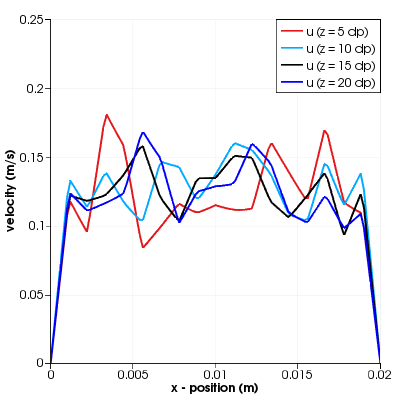
\includegraphics[width=\singleimagewidth]{chapters/figures/lbm/evap-u-profiles}
%     \caption{Velocity profiles (in the $x$-direction) at varying pebble bed heights for the pebble bed with 10\% damaged pebbles.}\label{fig:lbm-evap-u-profile}
% \end{figure}

\begin{figure}[t]
    \centering
    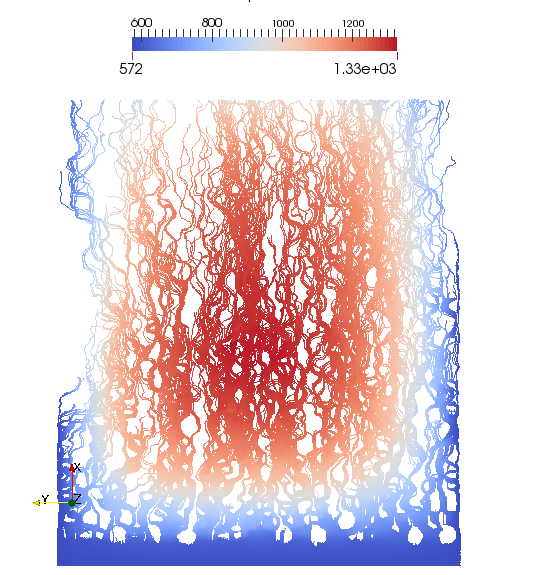
\includegraphics[width=\singleimagewidth]{chapters/figures/lbm/lbm-streamlines}
    \caption{Demonstrating the meandering path -- importantly wandering in the $x$-direction -- of fluid flow in the pebble bed.}\label{fig:lbm-streamlines}
\end{figure}

\begin{figure}[t]
    \centering
    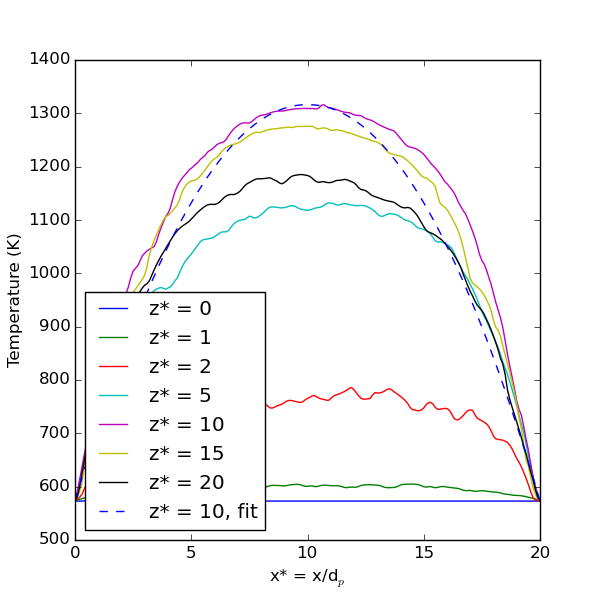
\includegraphics[width=\singleimagewidth]{chapters/figures/lbm/lbm-temp-profiles}
    \caption{Temperature profiles (in the $x$-direction) at varying pebble bed heights for the pebble bed with 10\% damaged pebbles. Shown for comparison is a parabolic profile that had fit both DEM and CFD-DEM temperature results.}\label{fig:lbm-temp-profiles}
\end{figure}

\begin{figure}[t]
    \centering
    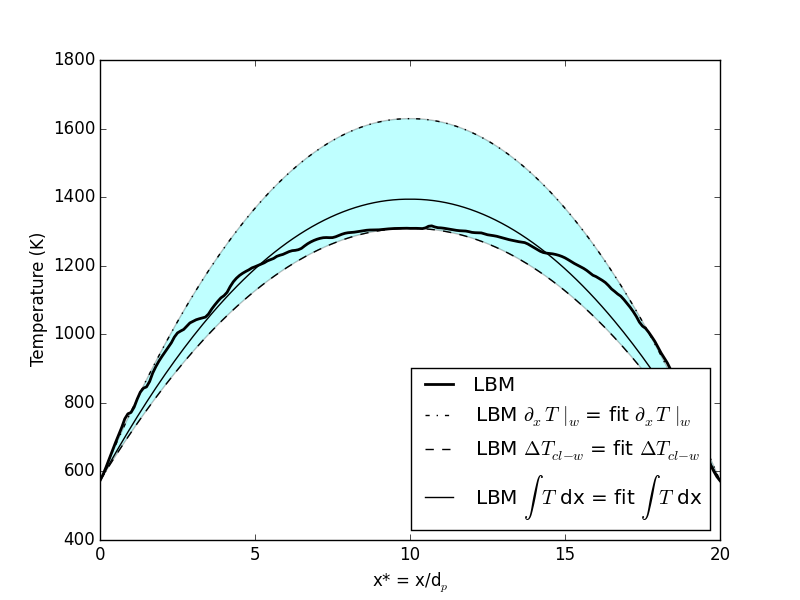
\includegraphics[width=\singleimagewidth]{chapters/figures/lbm/lbm-temp-profile_parabolic}
    \caption{Temperature profile from the LBM model is bound by parabolic curves. The LBM temperature profile increases sharply near the wall but then is flattened near the centerline. The behavior is indicative of laminar mixing of energy in the bed.}\label{fig:lbm-temp-parabolas}
\end{figure}

\begin{figure}[t]
    \centering
    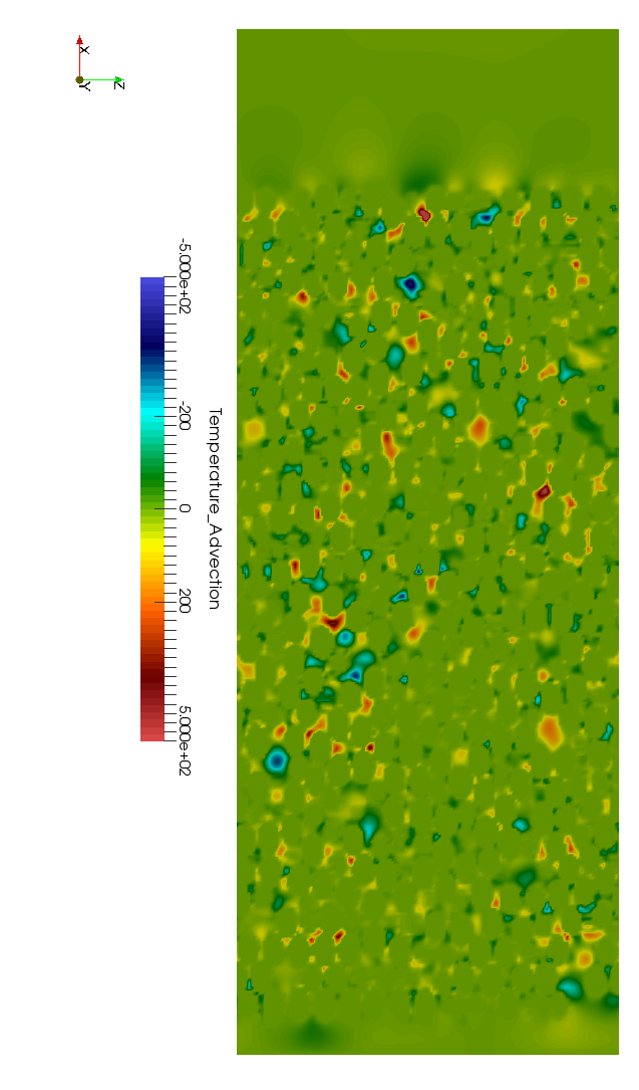
\includegraphics[width=\singleimagewidth]{chapters/figures/lbm/lbm-laminar-mixing}
    \caption{Slice of LBM simulation.}\label{fig:lbm-laminar-mixing}
\end{figure}

\FloatBarrier